\section{Aplicación de prueba}

\begin{subsection}{Parallel-Clusterer}
\begin{frame}\frametitle{Parallel-Clusterer}

\begin{block}{Parallel-clusterer}
Es una aplicación utilizada por la organización FuDePAN. Fue desarrollada utilizando el framework FuD y realiza la siguiente tarea:
\end{block}

\pause
\vspace{2mm}
\begin{block}{Tarea:}
Dado un conjunto de diferentes cadenas principales o esqueletos de una proteína (cada uno representado por un vector de átomos), agrupa estos elementos bajo similitudes geométricas de las posiciones de sus átomos.

El resultado final es un conjunto de agrupaciones o clusters donde cada uno tiene esqueletos de proteínas cuya estructura geométrica es muy similar.
\end{block}
\end{frame}

\begin{frame}\frametitle{Parallel-clusterer}

\textbf{Estructura de un esqueleto de proteína:}
\begin{center}
	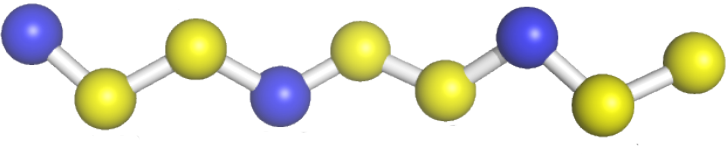
\includegraphics[scale=0.2]{images/backbone.png}
\end{center}

\textbf{Clusters resultantes:}

	\begin{minipage}{3cm}
		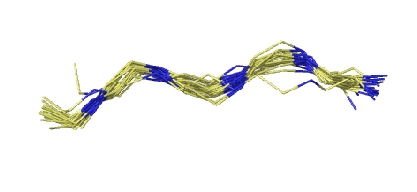
\includegraphics[scale=0.35]{images/grafico_cluster.jpg}
    \end{minipage}
    \    \ \hfill
	\begin{minipage}{5cm}
	    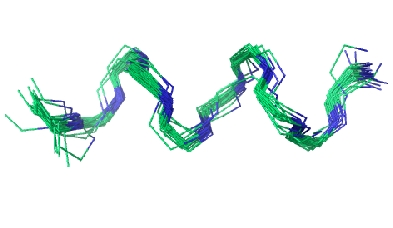
\includegraphics[scale=0.35]{images/grafico_cluster1.jpg}
	\end{minipage}
\end{frame}
\end{subsection}

\begin{subsection}{Análisis de rendimiento}
\begin{frame}\frametitle{Análisis de rendimiento}

\begin{block}{}
Es importante realizar el análisis de rendimiento de una aplicación distribuida con el propósito de estudiar los costos/beneficios que ésta posee ante la comparación con su versión secuencial.
\end{block}

\begin{block}{}
Se muestra el análisis de rendimiento de la aplicación Parallel-Clusterer compilada con FuD-BOINC en términos de las siguientes métricas:

\begin{itemize}
\item Aceleración
\item Eficiencia
\item Overhead
\item Costo
\end{itemize}

La ejecución se llevo a cabo variando de 1 a 5 clientes conectados.

\end{block}

\end{frame}

\begin{frame}\frametitle{Tiempo de ejecución}

\begin{block}{Tiempo secuencial (\textbf{$T_s$})}
Se define como el intervalo de tiempo que transcurre desde que un programa secuencial se inicia hasta que finaliza.
\end{block}

\pause
\begin{block}{Tiempo distribuido (\textbf{$T_p$})}
Se calcula desde que se inicia hasta que el último nodo finaliza su ejecución.
\end{block}

\pause
\begin{block}{}
Factores que afectaron al tiempo de ejecución de la aplicación distribuida:

\begin{itemize}
\item Tiempo de descarga de archivos de entrada y de la aplicación.
\item Tiempo de subida de los archivos resultantes.
\item Tiempo entre requerimientos al servidor.
\end{itemize}

\end{block}
\end{frame}

\begin{frame}\frametitle{Tiempo de ejecución}

\textbf{Tiempo secuencial (\textit{T$_{s}$}) vs. Tiempo paralelo (\textit{T$_{p}$})}

\vspace{2mm}
T$_{s}$ = 110.7 segundos.
\begin{center}
\begin{figure}[!ht]
    %Tabla & Grafico
    \begin{minipage}{2,0cm}
    \begin{flushleft}
    \begin{tabular*}{1,8cm}{c@{\extracolsep{\fill}}c}
        \hline
        \textbf{p} & \textbf{$T_p$} \\ \hline 
        1 & 305 \\ \hline
        2 & 249 \\ \hline
        3 & 259 \\ \hline
        4 & 245 \\ \hline
        5 & 222 \\ \hline
    \end{tabular*}
    \end{flushleft}
    \end{minipage}
    \    \ \hfill
    \begin{minipage}{8cm}
    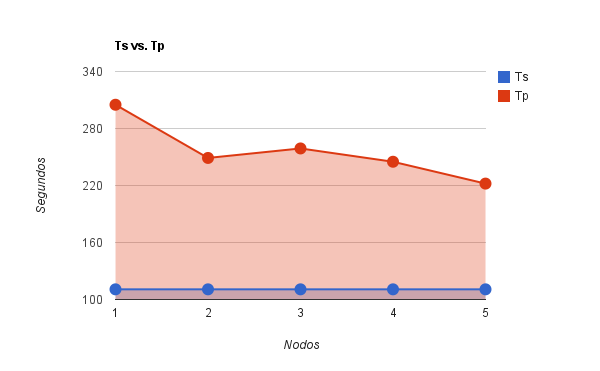
\includegraphics[scale=0.4]{images/Grafico_de_tiempos.png}\\
    \end{minipage}
\end{figure}
\end{center}
\end{frame}

\begin{frame}\frametitle{Aceleración}

\begin{block}{Definición}
Es una medida que arroja el beneficio relativo de resolver un problema en paralelo. Indica la ganancia de velocidad obtenida.
\end{block}

Se define como: \textit{S} = \textit{T$_{s}$}/\textit{T$_{p}$}

\begin{center}
\begin{figure}[!ht]
    %Tabla & Grafico
    \begin{minipage}{2,0cm}
    \begin{flushleft}
    \begin{tabular*}{1,8cm}{c@{\extracolsep{\fill}}c}
        \hline
        \textbf{p} & \textbf{$S$} \\ \hline 
        1  & 0.36 \\ \hline
        2  & 0.44 \\ \hline
        3  & 0.42 \\ \hline
        4  & 0.45 \\ \hline
        5  & 0.49 \\ \hline
    \end{tabular*}
    \end{flushleft}
    \end{minipage}
    \    \ \hfill
    \begin{minipage}{8cm}
    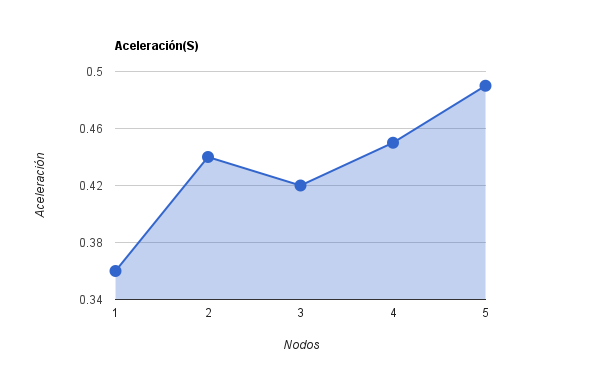
\includegraphics[scale=0.35]{images/Grafico_Aceleracion.png}\\
    \end{minipage}
\end{figure}
\end{center}

\end{frame}

\begin{frame}\frametitle{Eficiencia}

\begin{block}{Definición}
Indica el grado de utilidad de cada elemento de procesamiento.
\end{block}
Se define como: \textit{E} = \textit{S}/\textit{p}

\begin{center}
\begin{figure}[H]
    %Tabla & Grafico
    \begin{minipage}{2,0cm}
    \begin{flushright}
    \begin{tabular*}{1,8cm}{c@{\extracolsep{\fill}}c}
        \hline
        \textbf{p} & \textbf{$E$} \\ \hline 
        1  & 0.36 \\ \hline
        2  & 0,22 \\ \hline
        3  & 0,14 \\ \hline
        4  & 0,11 \\ \hline
        5  & 0,09 \\ \hline
    \end{tabular*}
    \end{flushright}
    \end{minipage}
    \    \ \hfill
    \begin{minipage}{8cm}
    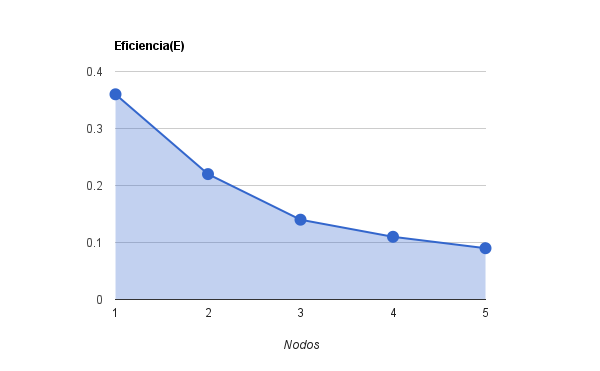
\includegraphics[scale=0.35]{images/Grafico_Eficiencia.png}\\
    \end{minipage}
\end{figure}
\end{center}

\end{frame}

\begin{frame}\frametitle{Overhead}

\begin{block}{Definición}
Indica el trabajo adicional que realiza un programa paralelo respecto a la solución secuencial equivalente.

\end{block}
Se define como: \textit{T$_{o}$} = \textit{p} $_*$ \textit{T$_{p}$} $_-$ \textit{T$_{s}$}

\begin{center}
\begin{figure}[H]
    %Tabla & Grafico
    \begin{minipage}{2,0cm}
    \begin{flushright}
    \begin{tabular*}{1,8cm}{c@{\extracolsep{\fill}}c}
        \hline
        \textbf{p} & \textbf{$T_0$} \\ \hline 
        1  & 194.3 \\ \hline
        2  & 387.3 \\ \hline
        3  & 666.3 \\ \hline
        4  & 869.3 \\ \hline
        5  & 999.3 \\ \hline
    \end{tabular*}
    \end{flushright}
    \end{minipage}
    \    \ \hfill
    \begin{minipage}{8cm}
    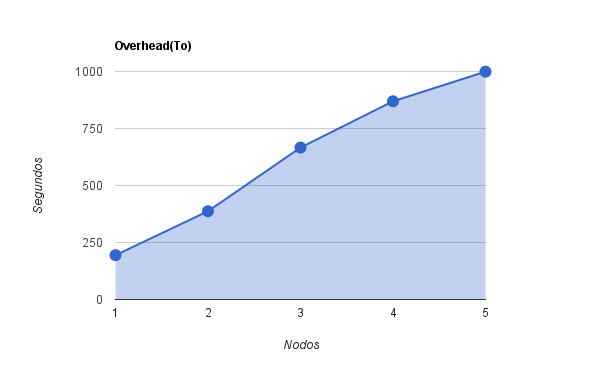
\includegraphics[scale=0.35]{images/Grafico_Overhead.png}\\
    \end{minipage}
\end{figure}
\end{center}

\end{frame}

\begin{frame}\frametitle{Costo}

\begin{block}{Definición}
Refleja la suma de los tiempos de ejecución de cada unidad de procesamiento.
\end{block}

Se define como: \textit{C} = \textit{p} $_*$ \textit{T$_{p}$}
\begin{center}
\begin{figure}[!ht]
	\begin{minipage}{2,0cm}
    \begin{flushright}
    \begin{tabular*}{1,8cm}{c@{\extracolsep{\fill}}c}
        \hline
        \textbf{p} & \textbf{$C$} \\ \hline 
        1  & 305 \\ \hline
        2  & 498 \\ \hline
        3  & 777 \\ \hline
        4  & 980 \\ \hline
        5  & 1110 \\ \hline
    \end{tabular*}
    \end{flushright}
    \end{minipage}
    \    \ \hfill
    \begin{minipage}{8cm}
    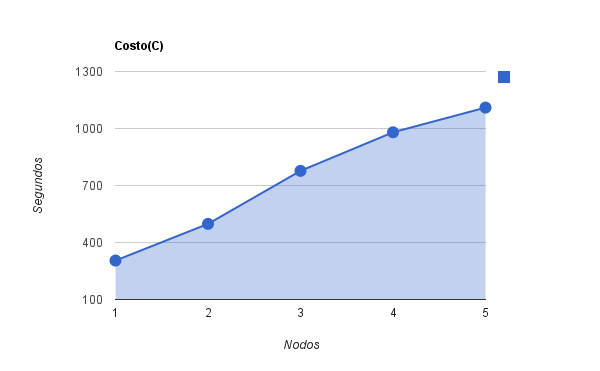
\includegraphics[scale=0.35]{images/Grafico_Costo.png}\\
    \end{minipage}
\end{figure}
\end{center}
\end{frame}

\begin{frame}\frametitle{Otros resultados: tiempos de ejecución}
\begin{center}
\begin{figure}[!ht]

	\begin{minipage}{3cm}
		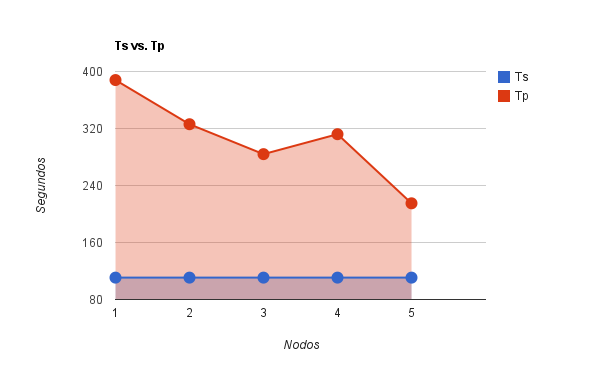
\includegraphics[scale=0.3]{images/grafico_de_tiempos1.png}
    \end{minipage}
    \    \ \hfill
	\begin{minipage}{5cm}
	    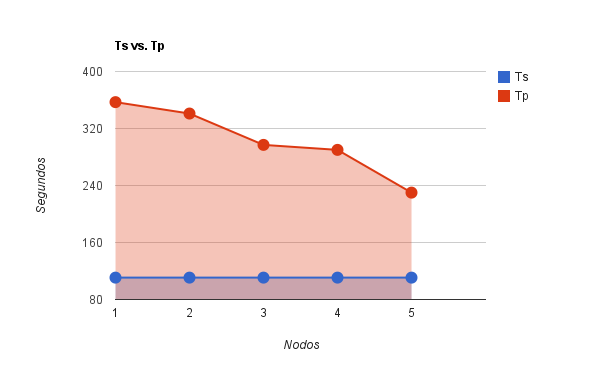
\includegraphics[scale=0.3]{images/grafico_de_tiempos2.png}
	\end{minipage}
\end{figure}
\end{center}

\end{frame}

\end{subsection}

